%%%%%%%%%%%%%%%%%%%%%%%%%%%%%%%%%%%%%%%%%
% a0poster Landscape Poster
% LaTeX Template
% Version 1.0 (22/06/13)
%
% The a0poster class was created by:
% Gerlinde Kettl and Matthias Weiser (tex@kettl.de)
% 
% This template has been downloaded from:
% http://www.LaTeXTemplates.com
%
% License:
% CC BY-NC-SA 3.0 (http://creativecommons.org/licenses/by-nc-sa/3.0/)
%
%%%%%%%%%%%%%%%%%%%%%%%%%%%%%%%%%%%%%%%%%

%----------------------------------------------------------------------------------------
%	PACKAGES AND OTHER DOCUMENT CONFIGURATIONS
%----------------------------------------------------------------------------------------

\documentclass[a0,landscape]{a0poster}
\usepackage{float}
\usepackage{multicol} % This is so we can have multiple columns of text side-by-side
%\usepackage{hyperref}
\columnsep=100pt % This is the amount of white space between the columns in the poster
\columnseprule=3pt % This is the thickness of the black line between the columns in the poster

\usepackage[svgnames]{xcolor} % Specify colors by their 'svgnames', for a full list of all colors available see here: http://www.latextemplates.com/svgnames-colors

\usepackage{titlesec}
\titlespacing\section{0pt}{12pt plus 4pt minus 2pt}{0pt plus 2pt minus 2pt}
\titlespacing\subsection{0pt}{12pt plus 4pt minus 2pt}{0pt plus 2pt minus 2pt}
\titlespacing\subsubsection{0pt}{0pt plus 4pt minus 2pt}{0pt plus 2pt minus 2pt}
\titlespacing\paragraph{0pt}{0pt plus 4pt minus 2pt}{0pt plus 2pt minus 2pt}

%%%%%%%% EDIT PAGE SIZE
\usepackage{pgfpages}
\makeatletter
\define@key{pgfpagesuselayoutoption}{18x24paper}[]
{\def\pgfpageoptionheight{18in} \def\pgfpageoptionwidth{24in}}
\makeatother
\pgfpagesdeclarelayout{resize and center}
{
  \def\pgfpageoptionborder{0pt}
}
{
  \pgfpagesphysicalpageoptions
  {%
    logical pages=1,%
    physical height=\pgfpageoptionheight,%
    physical width=\pgfpageoptionwidth%
  }
  \pgfpageslogicalpageoptions{1}
  {%
    resized width=\pgfphysicalwidth,%
    resized height=\pgfphysicalheight,%
    border shrink=\pgfpageoptionborder,%
    center=\pgfpoint{.5215\pgfphysicalwidth}{.47\pgfphysicalheight}%
  }%
}
\pgfpagesuselayout{resize and center}[18x24paper,landscape]

\usepackage{times} % Use the times font
%\usepackage{palatino} % Uncomment to use the Palatino font

\usepackage{graphicx} % Required for including images
\graphicspath{{figures/}} % Location of the graphics files
\usepackage{booktabs} % Top and bottom rules for table
\usepackage[font=small,labelfont=bf]{caption} % Required for specifying captions to tables and figures
\usepackage{amsfonts, amsmath, amsthm, amssymb} % For math fonts, symbols and environments
\usepackage{wrapfig} % Allows wrapping text around tables and figures

\begin{document}

%----------------------------------------------------------------------------------------
%	POSTER HEADER 
%----------------------------------------------------------------------------------------




% ====================
% Lengths
% ====================

% If you have N columns, choose \sepwidth and \colwidth such that
% (N+1)*\sepwidth + N*\colwidth = \paperwidth











% The header is divided into three boxes:
% The first is 55% wide and houses the title, subtitle, names and university/organization
% The second is 25% wide and houses contact information
% The third is 19% wide and houses a logo for your university/organization or a photo of you
% The widths of these boxes can be easily edited to accommodate your content as you see fit

\begin{minipage}[b]{0.80\linewidth}
\veryHuge \color{RoyalBlue} \textbf{Enhancing Stress Management and Mental Wellness in Bangladesh for Undergraduate Students through NLP and HCI} \color{Black}\\ % Title
% \Huge\textit{An Exploration of Complexity}\\[1cm] % Subtitle
\huge \textbf{MD Rifat Rahman (19101352), MD Mohibur Zaman (19101359), Mehbub Shifat ur Rasul (19101312),\\
MD Showrav Zaman (19101374), Mohyminul Islam Fahim (19101160)\\
Supervisor: Jannatun Noor, Assistant Professor} % Author(s)
\huge (Department of CSE, Brac University) % University/organization
\end{minipage}
%
% \begin{minipage}[b]{0.25\linewidth}
% \color{DarkSlateGray}\Large \textbf{Contact Information:}\\
% Department Name\\ % Address
% University Name\\
% 123 BroadwaAssNoore, Country\\\\
% Phone: +1 (000) 111 1111\\ % Phone number
% Email: \texttt{john@LaTeXTemplates.com}\\ % Email address
% \end{minipage}
%
\begin{minipage}[b]{0.15\linewidth}
\hspace{0.14\linewidth}

\includegraphics[width=12cm]{figures/bracu_logo.png} % Logo or a photo of you, adjust its dimensions here
\end{minipage}

\vspace{1cm} % A bit of extra whitespace between the header and poster content

%----------------------------------------------------------------------------------------

\begin{multicols}{4} % This is how many columns your poster will be broken into, a poster with many figures may benefit from less columns whereas a text-heavy poster benefits from more

%----------------------------------------------------------------------------------------
%	ABSTRACT
%----------------------------------------------------------------------------------------

\color{Navy} % Navy color for the abstract


\begin{abstract}

To address the mental well-being and stress management of undergraduates within the contemporary digital education landscape, characterized by increasingly significant challenges, this study seeks to establish a comprehensive system. This system will harmonize natural language processing (NLP) techniques for understanding emotions and language with human-computer interaction (HCI) principles for designing user-friendly interfaces. Furthermore, the study will employ both qualitative and quantitative research techniques, including qualitative interviews and quantity native surveys, to gain a holistic understanding of undergraduates’ mental health needs. In addition, snowball sampling will be employed to identify potential participants for the qualitative interviews, ensuring a diverse and representative sample. The integration of these research methodologies, along with the utilization of NLP
models such as BERT, RoBERTa, and DistilBERT, aims to equip undergraduates with valuable tools for self-reflection, emotional support, and effective stress management during their academic journey. This multifaceted approach will ultimately contribute to promoting a healthier and more productive undergraduate experience, accentuating the significance of user-centric HCI in addressing the well-being of students.
\end{abstract}


%----------------------------------------------------------------------------------------
%	INTRODUCTION
%----------------------------------------------------------------------------------------

\color{SaddleBrown} % SaddleBrown color for the introduction

\section*{Introduction}
Stress management and mental health promotion among Bangladeshi undergraduate students are urgent concerns in the fast-paced world of today. Technology is a major factor in the fast-changing global mental health landscape. The COVID-19 pandemic has significantly worsened stress, anxiety, and depression among university students, highlighting the need for creative solutions \cite{wang2020investigating}. The integration of machine learning with mental health services presents opportunities for early intervention that are both promising and ethically questionable \cite{thieme2020machine}. The importance of doing ethical and culturally sensitive research is highlighted by our focus on Bangladesh, which has a distinct sociocultural setting and presents unique obstacles for students. Given cultural quirks and socioeconomic circumstances, the nexus between human-computer interaction (HCI) and mental health research is important (Reference: HCI and Mental Health in Diverse Cultural Contexts). Prioritizing affordability, usability, and accessibility in mental health treatments is essential as we set out on this road \cite{zhang2022natural}. Technology can change mental healthcare. Examples of this include Natural Language Processing (NLP), Human-Computer Interaction (HCI), and sophisticated instruments (Reference: Technological Advancements in Mental Health Care). Harnessing the potential of technology for a more supportive and inclusive society requires collaboration between HCI specialists and mental health practitioners \cite{doherty2010design}


%\begin{center}\
%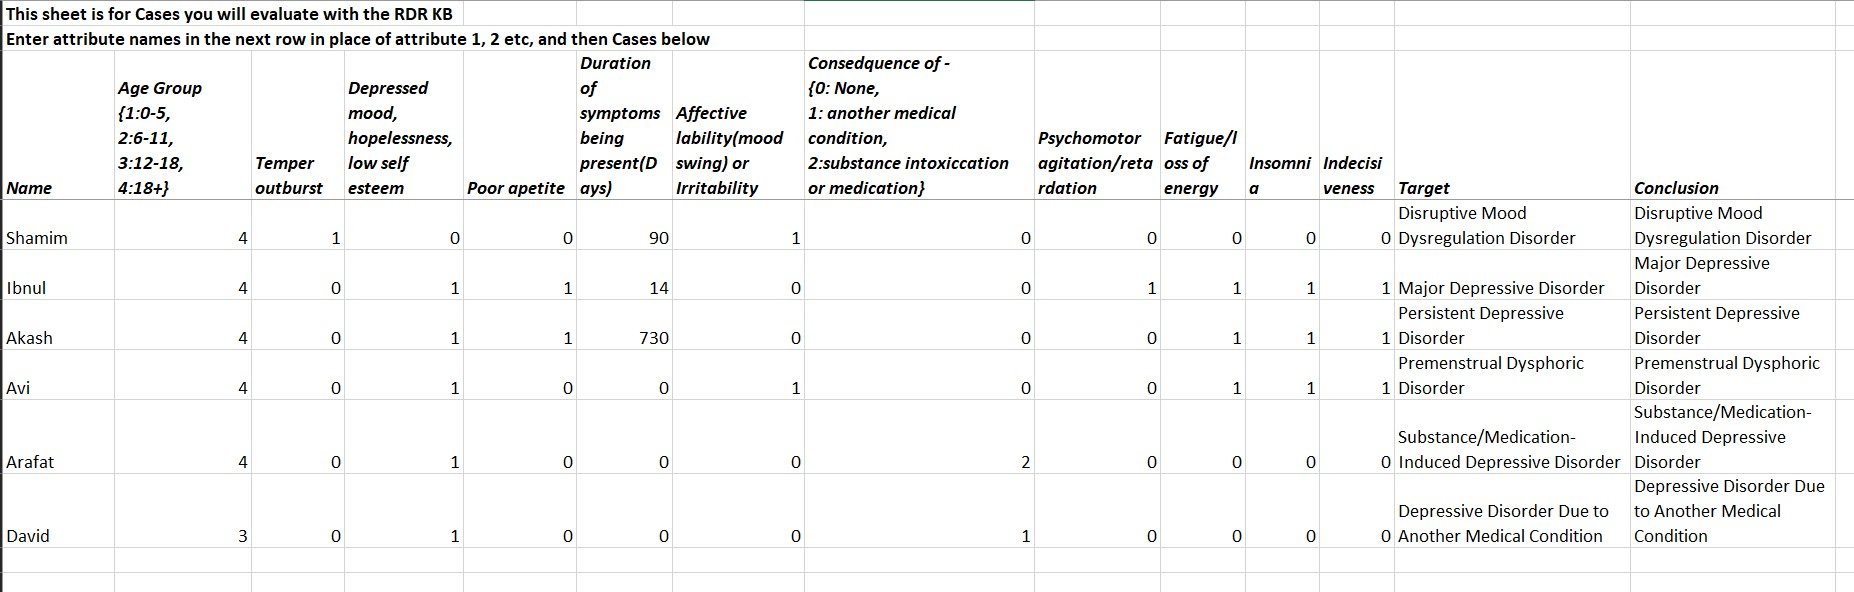
\includegraphics[width=0.8\linewidth]{rdr_model1}
%\captionof{figure}{\color{Green} Ripple Down Rules System Interface 1}
%\end{center}



%----------------------------------------------------------------------------------------
%	OBJECTIVES
%----------------------------------------------------------------------------------------

\subsection*{Problem Statement}
\begin{enumerate}
\itemsep-0.2em 
  \item Traditional approaches fall short most of the time during mental health diagnosis
  \item There is an absence of thorough research on the integration of technology and Human-Computer Interaction (HCI) for digital mental health interventions.
  \item It is difficult to design technology-driven mental health treatments since these factors must be improved: affordability, effectiveness, accessibility, and engagement.
\end{enumerate}

\subsection*{Research Objectives}
\begin{enumerate}
\itemsep-0.2em 

  \item Classifying Mental disorders.
  \item Based on the prediction provide a stress management solution.
  \item Provide a suggestion based on the user scenario.

            
\end{enumerate}


\color{DarkSlateGray} % DarkSlateGray color for the rest of the content




%----------------------------------------------------------------------------------------
%	MATERIALS AND METHODS
%----------------------------------------------------------------------------------------

\section*{Methodology}

For our research, we explore related public datasets. Based on analyzing the datasets preprocessing and model training were performed. Based on the performances, it was visible to us, that these datasets are not well fitted for our area of work. This leads us to create our own dataset and with the help of HCI, we prepare survey designs and questionaries for the survey and data collection. After collecting the data in our future work we will seek professional help to eliminate gaps of our not being expertized in mental health-related issues. This will help us to eliminate the gap between previous datasets and ours. Last, of all, our survey data will be labeled with the help of the professionals, so that it can predict mental health properly, and later on we will test the dataset with the models that previously performed better with similar kinds of datasets. This flow of events is also shown in the flowchart below Figure 1.
 


\begin{center}
\begin{minipage}[t]{1\linewidth}
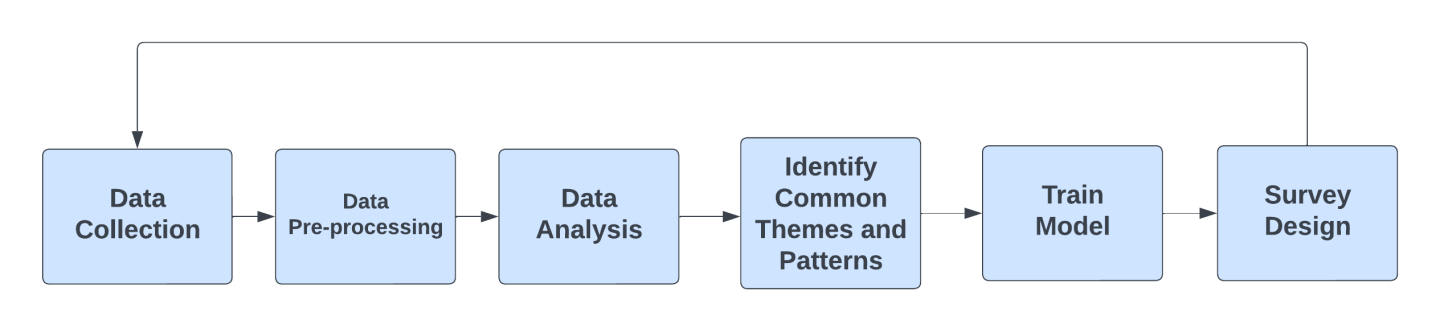
\includegraphics[width=\linewidth]{figures/Workflow_1.png} % Logo or a photo of you, adjust its dimensions here
\captionof{figure}{\color{Green} Methodology Pipeline}
\end{minipage}

\end{center}



%------------------------------------------------



%----------------------------------------------------------------------------------------
%	RESULTS 
%----------------------------------------------------------------------------------------

\section*{Datasets Analysis}

Based on the gathered Datasets some relatable parameters are being extracted. The dataset provides us with valuable parameters that serve as the foundation for crafting a well-structured survey design, which will enable us to formulate effective solutions for addressing mental health issues. interface is presented in Figure 2.
 


\begin{center}
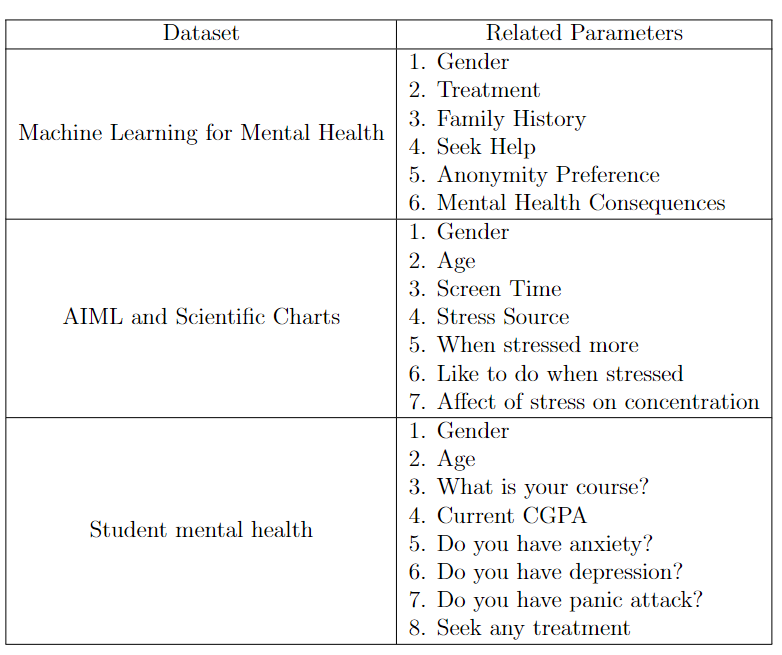
\includegraphics[width=0.5\linewidth]{figures/table.png}
\captionof{figure}{\color{Green} Related Parameters of the Datasets}
\end{center}

 %interface.\par
    





\section*{Preliminary Analysis}

\begin{center}\vspace{1cm}
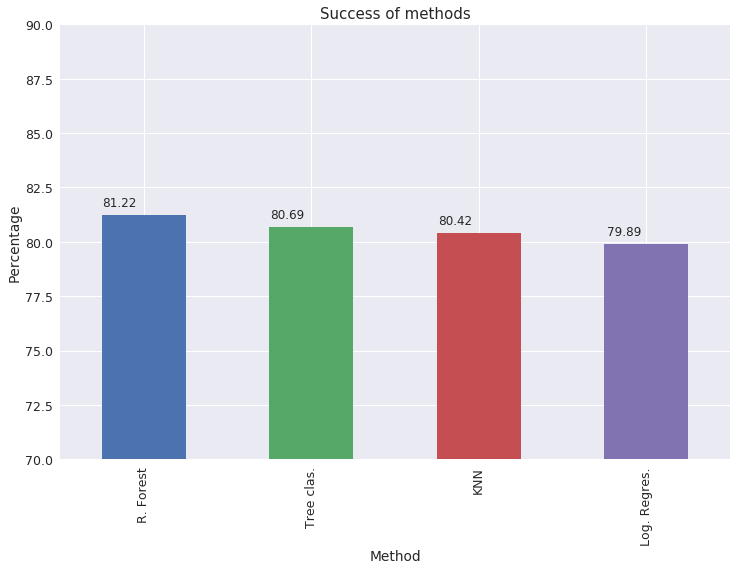
\includegraphics[width=0.7\linewidth]{figures/Dataset1.png}
\captionof{figure}{\color{Green} Result of Dataset 1}
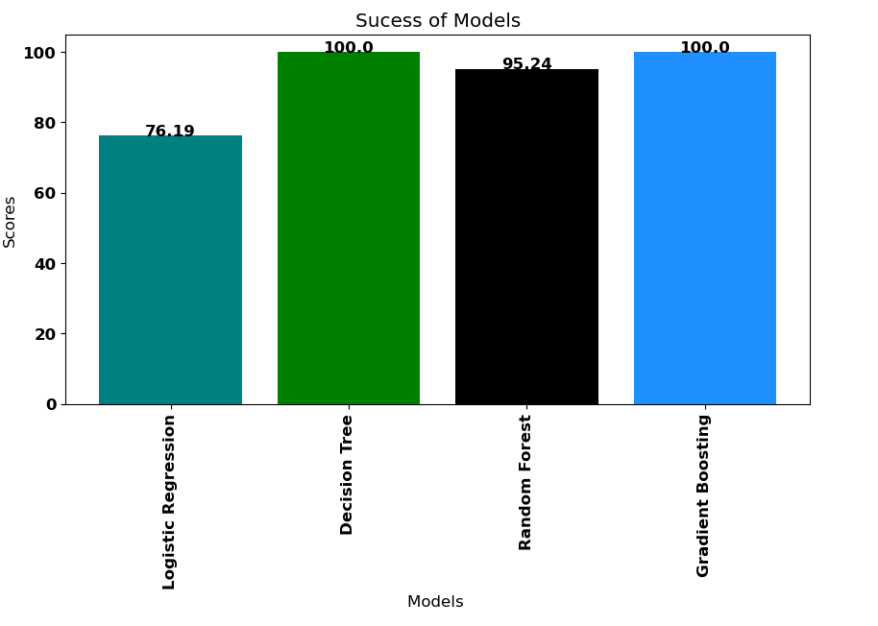
\includegraphics[width=0.7\linewidth]{figures/Dataset_2.png}
\captionof{figure}{\color{Green} Result of Dataset 2}
\end{center}\vspace{1cm}







\begin{table}[]
\centering
\begin{tabular}{|l|l|c|}
\hline
\multicolumn{1}{|c|}{Dataset}      & \multicolumn{1}{c|}{Applied Model}                                                                                                   & Accuracy                                                                        \\ \hline
Machine Learning for Mental Health & \begin{tabular}[c]{@{}l@{}}1. Logistic Regression\\ 2. K-nearest Neighbours (KNN)\\ 3. Random Forest\\ 4. Decision Tree\end{tabular} & \begin{tabular}[c]{@{}c@{}}1. 79\%\\ 2. 80\%\\ 3. 81\%\\ 4. 80\%\end{tabular}   \\ \hline
AIML and Scientific Charts         & \multicolumn{1}{c|}{-}                                                                                                               & -                                                                               \\ \hline
Student mental health              & \begin{tabular}[c]{@{}l@{}}1. Logistic Regression\\ 2. Decision Tree\\ 3. Gradient Boosting\\ 4. Random Forest\end{tabular}          & \begin{tabular}[c]{@{}c@{}}1. 76\%\\ 2. 100\%\\ 3. 100\%\\ 4. 95\%\end{tabular} \\ \hline
\end{tabular}
\caption{Applied Models on the Datasets}
\label{tab:my-table}
\end{table}







%----------------------------------------------------------------------------------------
%	CONCLUSIONS
%----------------------------------------------------------------------------------------

\color{SaddleBrown} % SaddleBrown color for the conclusions to make them stand out

\section*{Conclusions}

Overall for our research, we undertook an extensive data-gathering effort, which was
then followed by a thorough data preprocessing phase to ensure its suitability for
model training. Upon further examination of the datasets and careful analysis of
the results, it became apparent that the desired level of efficiency could not be fully
achieved given the limitations of our current resources. In light of the necessity for
a more comprehensive comprehension of the topic at hand, we have undertaken a
significant measure by formulating a survey design that is specifically suited to align
with our research aims. The chosen survey design exhibits potential for enhancing
our dataset by incorporating significant insights since we have strategically intended
to collect information that has been validated by mental health experts. The data
obtained from this comprehensive survey process will form the basis for an improved
model training phase in our final defence. The primary objective of our research is to
enhance and optimize the performance of our model, thereby enabling us to provide
comprehensive solutions for a wide range of mental health concerns. Ultimately,
the integration of factual data with sophisticated modeling tools will provide hold
the potential to unveil novel viewpoints and inventive strategies for tackling mental
health issues.












 %----------------------------------------------------------------------------------------
%	REFERENCES
%----------------------------------------------------------------------------------------
\color{DarkSlateGray}
\nocite{*} % Print all references regardless of whether they were cited in the poster or not
\bibliographystyle{plain} % Plain referencing style
\bibliography{Reference} % Use the example bibliography file sample.bib

%----------------------------------------------------------------------------------------
%	ACKNOWLEDGEMENTS
%----------------------------------------------------------------------------------------



%----------------------------------------------------------------------------------------

\end{multicols}
\end{document}